% !TEX root = ../../report.tex
\section{Evaluating Recommender Systems}
\label{sec:evaluation}

% Refering to research goals and defending why we need this section.
Our research \textbf{goals G5 and G8} requires us to identify existing metrics
for evaluating recommender systems in a sparse dataset with implicit feedback.
Set forth by our problem statement we need to propose one recommender system,
selected from a range of candidate approaches and techniques. We recall our
system overview in Figure~\ref{fig:app-overview} where in the last step of
the pipeline we \textit{evaluate} our recommendations. There are a range of
different metrics for ranking the performance of recommender systems, and they
are all highly dependent on which properties the system designer prioritizes as
important for both the domain and application.

% Explaining basic difference between offline/online eval.
There are mainly two settings for doing evaluation experiments. First is doing
them \textit{offline} where the system is evaluated without user interactions.
Second is, not surprisingly, \textit{online} evaluation, where real users
interact with the system. In this thesis we did not have the possibility to
perform any online evaluations, and hence a larger focus will be given to the
offline setting.

% Explain that evluations can guide us towards finding correct parameters.
It is important to note that having good evaluation metrics combined with
robust automation techniques are a crucial requirement in order to find the
optimal model-parameters. In most recommender models the number of free
parameters are high, and in order to best set them the designer need to first
select values based on intuition and experience. Later it is crucial to run
experiments fluctuating the parameter values until the optimal
\textit{evaluation score} is achieved.

% Refer to Appendix for more evaluation metrics, only focusing on suitable here.
There exists too many evaluation metrics to describe them all in this thesis,
consequently in this section will primarily focus on the ones suited for our
needs -- that is, extremely sparse implicit ratings in the fashion domain. A
comprehensive study of non-suitable solutions were performed as well, and can
be found in Appendix~\ref{appendix:evaluation-metrics}.

% Figure showing the various methods in evaluation.
\begin{figure}[H]
	\centering
	\begin{tikzpicture}[
		solid node/.style={
			draw,
			circle,
			inner sep=1.2,
			black
		},
		rec/.style={
			rectangle,
			draw,
			text width=2cm,
			text centered
		},
		edge from parent fork down,
		level 1/.style={level distance=25mm,sibling distance=45mm},
		level 2/.style={level distance=20mm,sibling distance=25mm}
	]
		\node [solid node] {}
			child{
				node [rec, align=center, sibling distance=10mm] {Implicit\\binary data}
				child { node[align=center] {Precision/\\Recall} }
				child { node[left=5mm] {MAP} }
				child { node[left=15mm] {AUC} }
				child { node[left=25mm] {Fallout} }
			}
			child{
				node [rec] {Explicit ground truth}
				child {
					node [rec] {Accuracy}
					child { node[left=15mm] {MAE}}
					child { node[left=15mm] {MSE}}
					child { node[left=18.5mm] {RMSE}}
				}
				child {
					node [rec] {Ranked}
					child { node[right=12mm] {AP Correlation}}
					child { node[right=15mm] {MPR}}
					child { node[right=15mm] {nDCG}}
				}
			}
			child{
				node [rec] {Live users}
				child { node[align=center, right=-5mm] {Multi-Armed\\Bandits} }
				child { node {A/B} }
			}
		;
	\end{tikzpicture}
    \caption{Overview of evaluation metrics based on input to recommender system}
	\label{fig:overview-eval}
\end{figure}

% Explain the figure and that we will refer to it. Mention that rightmost is
% online eval.
This figure shows an overview of the methods which \textit{will} be covered in
the following section, as well as functioning as a structure for the upcoming
discussion. As one can see the types of metrics used is highly dependent on
which type of data available. As one can see, the rightmost tree has live users
and is thus an online evaluation, whilst the remaining metrics are considered
in an offline environment. Various names and abbreviations will be explained as
we first analyze offline evaluation and look at the different methods in light
of the feedback from users being either explicit or implicit.

\subsection{Offline evaluation}

Offline experiments are performed using pre-collected datasets and a protocol
that models the user behavior to estimate recommender performance through
different evaluation measures. The following figure shows a \emph{traditional}
offline evaluation pipeline:

\begin{figure}[H]
		\centering
	  	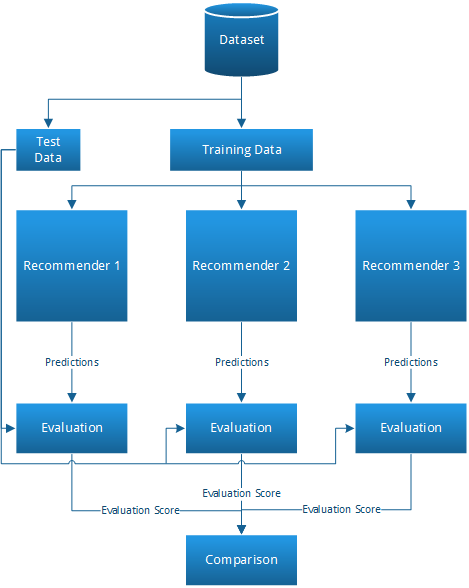
\includegraphics[scale=0.6]{image/evaluationpipeline.png}
		\caption[A Traditional Evaluation Pipeline]{A traditional evaluation pipeline for evaluating recommender systems}
		\label{figure:evaluationpipeline}
\end{figure}

Offline experiments are attractive because they require no interactions with
real users, and thus allows multiple researchers to compare a wide range of
algorithms, using the same data, at a low cost. The downside of offline
experiments is that they can answer a very narrow set of questions, typically
questions about the predictive power of the algorithm, and does not measure
other user factors.

In order to evaluate our metrics we need to establish a framework for testing,
defining how to interpret our results as well as how we utilize the dataset
with regards to both training and testing. There are two such methods, more
prevalent than others and which we use in this thesis, named \textit{the
holdout method} and \textit{K-fold cross-validation}.

Using the \textit{the holdout} method one split the dataset into two groups; a
training set used to train the classifier and a test set used to estimate the
error rate of the trained classifier. Both sets are equal for each test-run.
This is a useful technique in order to compare models based on the exact same
external factors, guaranteeing that the metrics obtained are a result of
model-parameters and not the training set. In addition this way of
\textit{holding out} the test set are often used in competitions and research
environments.

This method has two drawbacks: First, with sparse datasets we may not be able
to afford the luxury of setting aside a portion of the dataset for testing.
Second, since it is a single train-and-test experiment, the holdout estimate
can be misleading if we use a split not reflecting tendencies seen in the
actual training set.

The second method, \textit{K-fold Cross-Validation} builds on the holdout
methods by creating K partitions of the dataset. Then one runs $K$ experiments,
using $K-1$ partitions (or \textit{folds}) for training and the remaining one
for testing. One can easily see that setting $K=2$, makes this method
equivalent to the holdout method. The estimated error is found by taking the
average error from all the experiments.

\textit{Leave-one-out} is the degenerate case of K-fold Cross-Validation, where
$K$ is chosen as the total number of examples. For a dataset with $N$ examples
we perform $N$ experiments. For each experiment we use $N-1$ examples for
training and the remaining example for testing. Again, the true error is found
by taking the average error rate from the experiments.

In practice the number of folds often depends on the size of the dataset. For
large datasets, even 3-Fold Cross Validation will be quite accurate, which for
sparse datasets, one may wish to train as many examples as possible. In our
experiments we use $K$-values between $80$ and $200$, depending on model
selection and parameters.

The advantages of this methods are amongst many that the results are averaged
over the $K$ experiments. The strongest argument for using cross-validation is
the potential of using the entire training set iteratively for testing, creating
the largest possible test set for a fixed training data set.

The main disadvantage with K-fold Cross-Validation is the training algorithm
has to be run $K$ times, and thereby increasing the runtime for producing an
evaluation of the system. If the dataset is large, an increase of $K$ runs
could prove to be disadvantageous in time sensitive environments.

\subsubsection{Evaluation Mtrics: Prdictive Accuacy vs. Relevace}
When evaluating a recommender system, you wish to estimate a user's
satisfaction for a given recommendation. Traditionally recommender systems have
been evaluated by means of predictive accuracy. However, there is now a widely
agreed opinion that accurate predictions are crucial but insufficient to deploy
a good recommendation engine~\cite{Shani2011, McNee2006} as one also need to
consider the items \textit{relevance} and look at the set of recommendations as
a whole.  In addition, using implicit feedback we have no negative feedback and
our feedback does not indicate preference, but rather confidence of a users
opinion, thus calculating the predictive accuracy is not
efficient~\cite{Hu2008}

The three most common metrics for predictive accuracy are \textit{MAE},
\textit{MSE} and \textit{RMSE}. They measure how close the predicted ratings
are to the true user ratings (which we in SoBazaar does not explicitly have,
but are generated). More formally, the system tries to predict ratings
$\hat{r(c,i)}$ for a test set $T$ of user-item pairs $(c, i)$ for which the
true ratings are known.

The \textit{Mean Absolute Error (MAE)} measures how close the predictions are
to the actual outcome by:

\begin{equation}
    MAE = \frac{1}{n}\sum_{i=1}^{n}{|\hat{r(c,i)}-r(c,i)|}
    \label{equation:mae}
\end{equation}

where $r(c,i)$ is the actual outcome and $\hat{r}(c,i)$ is the predicted
value. As the name suggest, $MAE$ calculates the average absolute error.

The \textit{Root Mean Squared Error (RMSE)} is based on taking the square root
of the \textit{Mean Squared Error (MSE)} and they are both defined as:

\begin{equation}
    MSE = \frac{1}{n}\sum_{i=1}^{n}{(\hat{r(c,i)} - r(c,i))^{2}}
    \label{equation:mse}
\end{equation}

\begin{equation}
    RMSE = \sqrt{MSE}
    \label{equation:rmse}
\end{equation}

Where in Equation~\ref{equation:mse} $\hat{r(c,i)}$ is the predicted value and
$r(c,i)$ is the actual value. $RMSE$ is the square root of $MSE$ and is one of
the most used metrics to compare recommender algorithms in collaborative
filtering, and was the main metric used in the Netflix price competition to
evaluate the performance of the competitors recommender systems. As seen by the
equations, $RMSE$ is always bigger or equal to $MAE$, since $RMSE$ penalizes
errors more than $MAE$.

\subsubsection{Relevance based metrics}
\label{subsubsec:relevancemetrics}
Recommender system does not
predict the user's preferences of items, but tries to recommend to users items
that they may use. This is often done by giving the user a top-K set of
recommendations. Then using a dataset consisting of items each user has
used/interacted with, we select a test user and hide some of its interactions.
Finally we ask the recommender to predict a set of items which the user will
interact with, where the response is classified as one of four possible
outcomes:

\begin{table}[H]
	\centering
	\begin{tabular}{lll}
	\toprule
	-								&	Relevant						&	Not Relevant 				\\
	\midrule
	Recommended			&	True-Positive (TP) 	&	False-Positive (FP)	\\
	Not Recommended	&	False-Negative (FN)	&	True-Negative (TN)	\\
	\bottomrule
	\end{tabular}
    \caption[Usage prediction (Confusion Matrix)]{This table is showing the different categories recommended items can end up in.}
	\label{table:usageprediction}
\end{table}

\noindent
where the outcomes are defined as:

\begin{itemize}
	\item \textit{True-Positive (TP)}: The recommended item is of interest to the
	user.
	\item \textit{False-Positive (FP)}: The recommended item is not of interest to
	the user.
	\item \textit{False-Negative (FN)}: The item is of interest to the user, but is
	not recommended.
	\item \textit{True-Negative (TN)}: The item is not of interest to the user, but
	is not recommended.
\end{itemize}

This model assumes that if a non-relevant item never can be relevant. That is,
if a non-relevant item is recommended to a user, the item will never be
relevant for he/she. This assumption may be false, for example a user may
have been unaware of an items existence, but after the recommendation exposed
that item, the user can decide to select it. As a result no evaluation metric
is perfect, and there are compromises to be made between all methods. As we
will see in the discussion, one have to look at several metrics and come to a
joint reasoning based on multiple results. When items has been classified as
per Table~\ref{table:usageprediction} we can utilize a range of different
methods where the most common are \textit{Precision}, \textit{Recall},
\textit{Fallout} and \textit{MAP}, as seen in Figure~\ref{fig:overview-eval}.

\textit{Precision} is the fraction of retrieved items that are relevant.

\begin{equation}
    Precision = \frac{TP}{TP+FP}
    \label{equation:precision}
\end{equation}

Precision takes all recommended items into account, but it can also be
evaluated at a given cut-off point, only considering the top $n$ results
returned. This measure is called precision at n or P@n.

\textit{Recall} is the fraction of the items that are relevant to that are
successfully recommended.

\begin{equation}
    Recall = \frac{TP}{TP+FN}
    \label{equation:recall}
\end{equation}

Recall can therefore be seen as the probability that a relevant item is
retrieved by the recommender.

\textit{Fallout} is the amount of retrieved items which is not relevant amongst
all the non relevant items (false positive).

\begin{equation}
    Fallout = \frac{FP}{FP+TN}
    \label{equation:fallout}
\end{equation}

Fallout can therefore be looked at as the probability that a non-relevant item
is recommended.

\textit{F-measure} combines the precision and the recall.

\begin{equation}
    F_\beta = \frac{(1 + \beta^2) * (Precision * Recall)}{(\beta^2 * Precision + Recall)}
    \label{equation:f-measure}
\end{equation}

Based on the value of $\beta$ F-measure will weight precision or recall more.
For a $\beta$ over 1 F-measure will emphasize precision over recall, and
opposite for $\beta$ between 0 and 1.

\textit{Accuracy} is the amount of correctly recommended items over all the
items.

\begin{equation}
    Accuracy = \frac{TP+TN}{TP+TN+FP+FN}
    \label{equation:accuracy}
\end{equation}

\textit{Receiver Operating Characteristics (ROC)} is the recall rate ($TPR$)
against the fallout rate ($FPR$).  The goal is to maximize the recall while
minimizing the fallout.

\begin{equation}
    TPR(T) = \int_T^\infty P_0(T)dT
    \label{equation:tpr}
\end{equation}

\begin{equation}
    FPR(T) = \int_T^\infty P_1(T)dT
    \label{equation:fpr}
\end{equation}

$T$ is a threshold parameter.  The ROC curve is $TPR$ plotted together with
$FPR$ at various $T$.

\textit{Mean Average Precision (MAP)}~\cite{Manning:2008:IIR:1394399} measures
quality across recall levels.

\begin{equation}
	ap@n = \sum_{k=1}^{n}{\frac{P(K)}{min(m,n)}}
	\label{equation:apn}
\end{equation}
\begin{equation}
	MAP@n = \sum_{i=1}^{N}{\frac{ap@n_i}{N}}
	\label{equation:map}
\end{equation}

\ref{equation:apn} calculates the average precision at $n$ for a user.  From
\ref{equation:apn}, $P(K)$ is the precision at $k$ in the item list, $n$ is the
maximum number of predicted items and $m$ is the actual length of the predicted
items list. Equation~\ref{equation:map} calculates the mean of all the values from
\ref{equation:apn}.

Consider the following examples where we have three lists of hidden items and
three recommendations lists. All none relevant items are labeled with the item-id $0$.

\begin{table}[H]
\label{table:ap}
\centering
\begin{tabular}{*{4}l}
\toprule
Example 	& 	Actual					& 	Recommended					&	AP@10   \\ \midrule
1			& [1,2,3,4,5,6,7,8,9,10]	&	[1,0,0,0,0,0,0,0,0,0]		&	0.100  \\
2			& [1,2,3,4,5,6,7,8,9,10]	&	[1,0,0,0,2,0,0,0,0,0]		&	0.140  \\
3			& [1,2,3,4,5,6,7,8,9,10]	&	[8,0,0,0,9,0,0,0,0,0]		&	0.140  \\
4			& [1,2,3,4,5,6,7,8,9,10]	&	[1,0,0,0,3,0,5,0,0,0]		&	0.183  \\
5			& [1,2,3,4,5,6,7,8,9,10]	&	[0,0,0,2,0,0,0,6,5,0]		&	0.083  \\
6			& [1,2,3,4,5,6,7,8,9,10]	&	[0,0,0,0,7,0,8,0,0,0]		&	0.049  \\
7			& [1,2,3,4,5,6,7,8,9,10]	&	[0,0,0,0,7,0,0,0,0,1]		&	0.040  \\
8			& [1,2,3,4,5,6,7,8,9,10]	&	[0,0,0,0,0,0,0,8,5,0]		&	0.035  \\
9			& [1,2,3,4,5,6,7,8,9,10]	&	[1,3,4,5,6,0,0,0,0,0]		&	0.500  \\
10			& [1,2,3,4,5,6,7,8,9,10]	&	[0,0,0,0,0,1,2,8,5,3]		&	0.178  \\
\bottomrule
\end{tabular}
\caption{$AP@10$ Examples}
\end{table}

As you see from example two and three average precision does not consider the order of the actual item list
as all items are seen as equally relevant.

\begin{equation}
    AUROC = \int_\infty^{-\infty} TPR(T)P_0(T)dTdT
    \label{equation:auroc}
\end{equation}

Equation~\ref{equation:auroc} can be used to calculate the area under the
curve.  $AUROC$ is the probability that the recommender system will rank
positive examples higher than negative examples.  The Area Under is a commonly
used evaluation method for binary choice problems. If somebody makes random
guesses, the ROC curve should be a diagonal line stretching from (0,0) to
(1,1), as shown by the blue line in the figure below, scoring an AUC of 0.5. A
perfect model will score an AUC of 1.0. In practice, almost all models will fit
somewhere in between. One therefore obviously  aims to maximize the area under the
curve (AUC). The higher up all relevant items (true positives) are in the recommendation list,
the higher the AUC score. AUC can therefore be used as a single measure for the overall
quality of a recommender system.

\marginpar{TODO: Make Fit}

\begin{figure}[H]
\label{fig:aucroc}
  \centering
    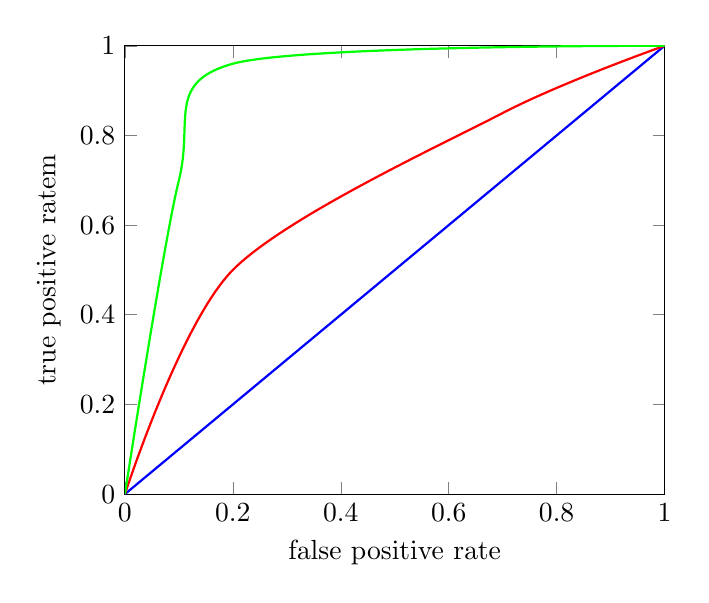
\begin{tikzpicture}
      \begin{axis}[
      	xlabel={false positive rate},
      	ylabel={true positive ratem},
      	ymin = 0, ymax=1, xmin=0, xmax=1,
      ]
      \addplot[thick,smooth,blue]{x};
      \addplot[thick,smooth,red] plot coordinates {
              (0,0)
              (0.2,0.5)
              (0.7,0.85)
              (1,1)
          };
      \addplot[thick,smooth,green] plot coordinates {
                    (0,0)
                    (0.1,0.7)
                    (0.2,0.96)
                    (1,1)
                };
      \end{axis}
    \end{tikzpicture}
    \caption{ROC curves}
\end{figure}

\subsubsection{Limitations of relevance based metrics}
\label{subsec:limitations-relevancebased}

The following table shows an example of the AUC values when varying the position of a single relevant document through the
recommendation list.

\begin{table}[H]
	\centering
	\begin{tabular}{*{12}l}
	\toprule
	\#Example	& R1 & R2 & R3 & R4 & R5 & R6 & R7 & R8 & R9 & R10 & AUC \\ \midrule
	1		& \cmark & \xmark & \xmark & \xmark & \xmark & \xmark & \xmark & \xmark & \xmark & \xmark & 1.000 \\
	2		& \xmark & \cmark & \xmark & \xmark & \xmark & \xmark & \xmark & \xmark & \xmark & \xmark & 0.889 \\
	3		& \xmark & \xmark & \cmark & \xmark & \xmark & \xmark & \xmark & \xmark & \xmark & \xmark & 0.778 \\
	4		& \xmark & \xmark & \xmark & \cmark & \xmark & \xmark & \xmark & \xmark & \xmark & \xmark & 0.667 \\
	5		& \xmark & \xmark & \xmark & \xmark & \cmark & \xmark & \xmark & \xmark & \xmark & \xmark & 0.556 \\
	6		& \xmark & \xmark & \xmark & \xmark & \xmark & \cmark & \xmark & \xmark & \xmark & \xmark & 0.444 \\
	7		& \xmark & \xmark & \xmark & \xmark & \xmark & \xmark & \cmark & \xmark & \xmark & \xmark & 0.333 \\
	8		& \xmark & \xmark & \xmark & \xmark & \xmark & \xmark & \xmark & \cmark & \xmark & \xmark & 0.222 \\
	9		& \xmark & \xmark & \xmark & \xmark & \xmark & \xmark & \xmark & \xmark & \cmark & \xmark & 0.111 \\
	10		& \xmark & \xmark & \xmark & \xmark & \xmark & \xmark & \xmark & \xmark & \xmark & \cmark & 0.000 \\
	\bottomrule
	\end{tabular}
	\caption{AUC Example - Varying the position of a single relevant in the recommendation list}
	\label{table:auc}
\end{table}


As mentioned by Powers et al.~\cite{powers2007}, recall, precision, F-measure
have a bias.  Recall, precision and F-measure ignore performance in correctly
handling negative examples, they propagate the marginal prevalences and biases,
and they fail to take account the chance level performance.  Another drawback
or limitation with the measuring of user predictions is that it does not take
into account the ranking of the items. To handle this, rank based metrics can
be used.

\subsubsection{Rank Based Evaluation Metrics}
\label{subsubsec:rankbased}

Rank accuracy metrics measure the ability of a recommendation method to produce
a recommended ordering of items that matches how the user would have ordered
the same items. Shani et al.~\cite{Shani2011} lists two different approaches
for measuring the ranking accuracy: Try determining the correct order of a set
of items for each user and measure how close a system comes to this correct
order, or we can attempt to measure the utility of the system's ranking to a
user.

Herlocker et al.~\cite{Herlocker2004} argue that rank accuracy metrics may be
overly sensitive for domains where the user just wants an item that is `good
enough' (binary preferences) since the user won't be concerned about the
ordering of items beyond the binary classification. These metrics are therefore
most suitable to evaluate algorithms that are used to present ranked lists to
the user in domains where the user preferences are expressed using numerical
values.

\marginpar{TODO: Leave or let be?}
The recommendation lists can also consist of several items with similar rating that
can appear in varying orders.
Since the user can express the same rating for similar
items, the list will again contain groups of items that can appear in arbitrary order.
The bottom line is that in most cases a rank metric for partial ordering would be more
appropriate for comparing recommendation lists that are produced by recommenders to item
rankings from known user preferences.

As we do not have explicit data in SoBazaar per Figure~\ref{fig:overview-eval}
we will not explore these methods in detail, however we will list some of the
most common ones. Note that although \textit{MAP} is defined as being a
relevance based metric used with implicit ratings, it does produce a ranked
list. It is however described in Section~\ref{subsubsec:relevancemetrics} and not here, as it does not
compare two ranked lists as the methods below does.

% todo maybe structure:
% precision - ranked list - explicit - human interaction

Two naïve ways of measuring how well to lists compare is to see how many items they have in common or how many of the items in the lists have the same rank. AP correlation is more sophisticated than this, and is the next measuring method described.

\textit{AP correlation}~\cite{Yilmaz:2008:NRC:1390334.1390435} measures the
overall precision and is a variant of \textit{Kendall's tau}.  It counts the
amount of items correctly placed in a ordered predicted rank list
\textit{list1} and a list of the actual rank ordering of the preferences of the
user \textit{list2}.

\begin{equation}
	AP = \frac{2}{N - 1} * \sum_{i=2}^{N}{(\frac{C(i)}{i - 1})} - 1
	\label{equation:ap}
\end{equation}

where $C(i)$ is the number of items ranked correctly above rank $i$.
The value of AP is between -1 and 1, where a score of 0 means that
\textit{list1} can be considered a randomly generated list and 1 is a perfect
match with the actual list \textit{list2}.

When measuring the rank of an item, the other items' rank is crucial, the next measurement gives the rank of an item based on its position amongst a random recommended ranked subset of the data.

\textit{Mean Percentage Ranking (MPR)} is a recall-oriented metric.  A known
issue with implicit feedback is that it often lack the actual user's
preference.  This approach is used to measure the user satisfaction of items in
an recommended ordered list.

\begin{equation}
	MPR = \frac{\sum_{u,i}{r_{ui} * rank_{ui}}}{\sum_{u,i}{r_{ui}}}
	\label{equation:mpr}
\end{equation}

How to calculate $MPR$ is shown in~\ref{equation:mpr}.  A list of all the items
for user $u$ is ordered based on the rank $rank_{ui}$ of the $u$.  Where
$rank_{ui}$ is the percentile rank of item $i$ in this list for $u$.
$rank_{ui} = 0$ means that $i$ is the most preferred item for $u$.  $r_{ui}$
indicates whether $u$ has consumed $i$ or not.  This makes a $MPR$ value of
0\% to be the most preferred value, and a value of 50\% meaning a near
randomly produced list.

After having looked at \emph{MPR} we will move over to \emph{nDCG}.

\textit{Normalized Discounted Cumulative Gain (nDCG)} measures the graded
relevance of the recommended item, the ranking quality or the usefulness of the
recommended item based on its rank position.  It is often used to measure the
performance of web search recommendation systems.

\begin{equation}
    DCG_k = \sum_{i=1}^{k}{\frac{2^{rel_i}-1}{log_2(i+1)}}
    \label{equation:dcg}
\end{equation}

\begin{equation}
    nDCG_k = \frac{DCG_k}{IDCG_k}
    \label{equation:ndcg}
\end{equation}

How to calculate the $nDCG$ value is shown in~\ref{equation:ndcg}.  Where $k$
is the maximum amount of suggested items, and $rel_i$ is the graded relevance
of the result at position $i$.  $IDCG_k$, from~\ref{equation:ndcg}, is the
ideal $DCG_k$ value.  This is the result list sorted on relevance.

% intro HLU
There are other ways of measuring how well a ranking algorithm performs based on the positions of relevant items in a list, \emph{HLU} is another way of doing so.

\textit{Half-life utility}~\cite{Breese:1998:EAP:2074094.2074100} assume that
the further down an item is in the list the less chance there is for that item
to be viewed by the user.  The rate of the decaying probability is exponential.

\begin{equation}
	HL_u = \sum_{i}{\frac{\delta(i)}{2^{\frac{i-1}{\alpha-1}}}}
\end{equation}

$\delta(i)$ is 1 if the user is interested in the item at position $i$ and 0 if
not.  $\alpha$ is the viewing half-life, or half-life parameter.  The half-life
utility of all the users are shown in~\ref{equation:HL}

\begin{equation}
	HL = 100 * \frac{\sum_u{HL_u}}{\sum_u{HL_u^{max}}}
	\label{equation:HL}
\end{equation}

where $HL_u^{max}$ is the maximum possible value of the half-life utility
value.

One issue with using a ranked based approach is that the items in the predicted
top K list has to be ranked in some way, the same goes for the list this list
is to be compared to.  Thereby producing the requirement for a ranked list of
preferred items from the user.  If there is such a ranked list, ranking
accuracy will help to tell how well the system is suggesting items for the
user, such as~\cite{Yilmaz:2008:NRC:1390334.1390435}.

\subsubsection{Global metrics - evaluating recommendation properties}

There is an emerging understanding that good recommendations accuracy alone
does not give the users of the recommender system an effective and satisfying
experience \cite{Herlocker2004}. The following \emph{measures} attempts to
assess a recommender systems usefulness beyond being able to provide accurate
recommendations to the users. These metrics are important whether one have
explicit, implicit or live users as input the the recommender system.

\textit{Coverage} can refer to several distinct properties of the system. Most
commonly, the term coverage refers to the proportion of items the
recommendation system can recommend, also known as \emph{item-space coverage}.
The simplest measure of catalog coverage is the percentage of all items that
can ever be recommended. Coverage can also be the proportion of users
interactions for which the system can recommend items, known as
\emph{user-space coverage}. In many applications the recommender system may not
provide recommendations for some users due to e.g.\\ low confidence in the
accuracy of predictions for that user. In such cases one may prefer a
recommender that can provide recommendations to a wider range of users.
However, an increase in coverage is only beneficial if the accuracy does not
drop significantly.

\textit{Perceived quality} is measured by first asking the user to examine the
recommended item, and give feedback regarding the their actual interest in the
recommended item.  For the feedback from the user to be as complete as
possible, the system must supply the user with the reason to why the item was
suggested, and the metadata of the item.  When the user has this overview of
the item, the user's feedback regarding the item can produce some quality
measure.  One  way of having the user to give this feedback is to re-rate the
recommended item on a similar scale as the item was rated.  A rating scale from
1 to 5 is often used for both~\cite{Schafer:1999:RSE:336992.337035}.

\textit{Novelty and Serendipity} are described in in
Section~\ref{subsec:rec-challenges}. We saw that novelty is expected to change
over time, some times the user would like to receive recommendation on new
items, and other times recommendations closer to the user's preferences.  For
the system to be able to detect these changes in preferences, and acting
accordingly would be beneficial in regards of the user's satisfaction.

\begin{equation}
    Novelty(u) = \frac{1}{N}\sum_{i=1}^{N}{1 - Knows(u,i)}
    \label{equation:novelty}
\end{equation}

In~\ref{equation:novelty} $Knows(u,i)$ represents a binary functions which
returns 1 if the user $u$ knows the item $i$, and 0 if not.  The set of items
used for the calculation is the set of recommended items for the user.

The system should be able to produce items both items known to the user, and
items unknown to the user.  For trust in the system and novelty respectively.

Measuring serendipity can be done though measuring how hard the prediction was
to do~\cite{serendipity}.  The metric used by~\cite{serendipity} bases its
assumptions on the idea that unexpectedness is low for \emph{easy-to-predict}
items, and high for \emph{difficult-to-predict} items.  To calculate how easy a
prediction is~\cite{serendipity} introduces a primitive prediction method and
compare the predictions done by this recommender, with the results from their
more sophisticated recommender, which serendipity is to be calculated for.
Unexpectedness is then the deviation from the result obtained by the primitive
predictions method.

Unexpectedness is calculated in as shown in the equation below.

\begin{equation}
    unexpectedness = \frac{1}{N}\sum_{i=1}^{N}{max(Pr(s_i) - Prim(s_i),0) * isrel(s_i) * \frac{count(i)}{i}}
    \label{equation:serendipity}
\end{equation}

In equation~\ref{equation:serendipity} $Pr(s_i)$ is the prediction made by the
sophisticated method of item $s_i$ in a ranked list, and $Prim(s_i)$ is the
same for the primitive.  $isrel(s_i)$ is binary and indicated whether or not
the item is of interest for the user, and $count(i)$ is used to give more
weight to correct items higher in the list.

\textit{Diversity} is generally defined as the opposite of similarity. In some
cases suggesting a set of similar items may not be as useful for the user,
because it may take longer to explore the range of products. E.g. when
presenting a list of 5 recommendations, the system should not recommend 5 Ralph
Lauren shirts with different colors. As diversity may come at the expense of
other properties such as accuracy, one should evaluate the decrease in accuracy
vs. the increase in diversity.

Other evaluation methods worth knowing about includes confidence, trust,
utility, robustness, adaptivity, scalability mentioned in \cite{Herlocker2004,
Shani2011}.

\textit{User-Centric Evaluation} focuses on the perceived quality of the
recommendation system~\cite{Pu2011}.  To gather this kind of information, user
feedback is required.  User-centric evaluation is meant to handle the short
comings of the offline evaluation metrics, such as predictive accuracy metrics.
User-centric evaluation can make evaluations on items which the user has not
yet show interest in.  This allows user-centric evaluation to make evaluations
on information about the system, such as the perceived quality and novelty of
the recommendation system.  When the user feedback has been gathered the data
must be analyzed.

\subsubsection{Evaluation of Cold-start Recommendations}
\label{sec:cold-start-eval}

The cold-start problem can be considered a sub problem of coverage. The
cold-start problem occurs when the recommender system cannot draw any
inferences for user or items which it has not yet gathered sufficient
information. When evaluating the cold-start system performance one is
interested in measuring the system accuracy for these users and items.

The evaluation metric used depends on the type of feedback available.  Most
experiments carried out have used \emph{traditional} explicit feedback datasets
such as MovieLens, EachMovie, Netflix etc. Accuracy metrics such as
MAE~\cite{Rashid2002, Rashid2008, Massa2004, Massa2007, Stern2009} and
RMSE~\cite{Agarwal2009, Agarwal2010} are therefore the most used ones. In the
experiments where binary rating data have been used Precision@N~\cite{Liu2011,
Gantner2010}, ROC curves~\cite{Agarwal2009, Gantner2010, Schein2002} and Area
Under Curve (AUC) \cite{Liu2011, Gantner2010} seems to be the preferred
evaluation metrics.
Massa et al.~\cite{Massa2004} argue that performance measures such as Mean
Absolute User Error (MAUE) is a good measure for cold-start recommendations
since every user is taken into account once and a cold start user is as
influential as an heavy rater. Similarly, Park et al.~\cite{Park2006} measure
normalized MAE (NMAE) by macro-averaging, which first calculates the mean
average error of each users and taking the average of all users.
Another way to discriminate between different recommender techniques is
coverage. The recommender system may not be able to make predictions for every
item. For this reason, it is important to measure the portion of ratings that
an RS is able to predict (ratings coverage). However, this quantity is not
always informative about the quality of a recommender system. A RS is likely to
be good at predicting nearly all the ratings for heavy users and not be able to
do the same for users who have rated few items. For this reason, one should
also compute the users coverage, defined as the portion of users which the RS
is able to predict at least one rating for. Good et al.~\cite{Good1999}
measure the item-space coverage, while Massa et al.~\cite{Massa2004,
Massa2007} measures both the item-space coverage and user-space coverage of
their methods.

To simulate the cold-start scenario, different approaches have been employed:
One popular way to simulate a cold-start user scenario used by~\cite{Stern2009,
Lam2008} is to split the dataset in two disjoint sets, a training set
containing $90\%$ of the users and the remaining $0\%$ in the test set. For
each test user one trains a model with a random subset $T\%$ of their ratings
e.g.\ $5\%$ or $75\%$, and then use the model to predict their remaining
ratings. The same methodology can also be used to simulate a cold-start item
scenario. Another highly similar way to simulate the cold-start user and
cold-start item scenario was used in~\cite{Rashid2002, Rashid2008}. For the
cold-start user scenario one selects a subset of the users with e.g.\ more than
200 ratings. One then trains the model with a subset of the ratings. In the
case of~\cite{Rashid2002} 30, 45, 60 and 90 ratings was used. After training
the model one computes the error on the hidden ratings for the same user.
Stern et al.~\cite{Stern2009} also used a similar method which they called
Given $n$, in which they trained their model using 2, 5 and 10 ratings for each
test user and predict the remaining values.
The advantage of the latter approach is that they use a selection criteria for
the test users to avoid users with really few ratings which might be crucial on
a cold-start dataset. The obvious problem with this approach is that for
cold-start datasets these users might stand for a large portion of the ratings.
There are both pros and cons of using a fixed subset of ratings rather than
using the percentage of ratings, the best choice will most likely depend on the
dataset. Using a fixed subset of ratings would be preferable e.g. if the number
number of ratings given by the users are fairly uniform.

Another \emph{simpler} approach employed by~\cite{Massa2007, Jamali2009} is to
determine a cutoff point for what is considered a cold-start user. E.g.\ that
every user with less than 5 ratings is considered a cold-start user. Then
separately measure the error on predictions made to these users.

The problem with this approach is that it does not measure how well the
recommendation quality improves as more rating information becomes available,
giving a less detailed view of the systems performance. The actual number of
ratings predicted is also likely to be fairly small given a cold-start dataset.

To simulate a cold-start system scenario Agarwal et al.~\cite{Agarwal2009}
split the dataset in two using 75\% of the dataset for training and 25\% for
testing. They then train the model using 30\%, 60\% and 75\% of the data and
compare their performance on the testset. This model is both good and simple
as it measures the recommender systems quality for different sparsity levels.

%Summary of articles read

%	What evaluation metrics are used?

%\cite{Rashid2008}: Accuracy metric: MAE, Expected Utility (Penalize false positives more than false negatives)
%\cite{Rashid2002}: Accuracy metric: MAE
%\cite{Massa2004}: Leave one out, MAE, MAUE, Rating Coverage, User Coverage
%\cite{Massa2007}: Leave one out, MAE, MAUE, Rating Coverage, User Coverage,
%\cite{Jamali2009}: Leave one out, Recall/Hit-ratio
%\cite{Agarwal2009}: Movie: RMSE, Yahoo: ROC curves, 5-fold cross validation
%\cite{Agarwal2010}: RMSE, True Positive Rate, True Positive Rate
%\cite{Liu2011}: Precision at N, Mean average precision, area under curve
%\cite{Park2006}: NMAE
%\cite{Good1999}: Coverage, MAE, ROC
%\cite{Stern2009}: MAE
%\cite{Ganter2010}: Precision at N (5 & 10), AUC (General ranking measure)
%\cite{Schein2002}: GROC (hit/miss rate)

%	What type of user feedback is used?

%\cite{Rashid2008}: Explicit feedback, MOVIELENS, Only users with 80 or more ratings
%\cite{Rashid2002}: Explicit feedback, MOVIELENS, Only users with 200 or more ratings
%\cite{Massa2004}: Explicit feedback, EPINIONS + Web of trust
%\cite{Massa2007}: Explicit feedback, EPINIONS + Web of trust
%\cite{Jamali2009}: Explicit feedback, EPINIONS + Web of trust
%\cite{Agarwal2009}: Explicit feedback, MovieLens + EachMovie, also incorporates user features
%\cite{Agarwal2010}: Explicit feedback + User features and bag of words rep of crawled movie data - MovieLens, Yahoo! Buzz (1 or -1), BookCrossing
%\cite{Liu2011}: Explicit feedback. Netflix...
%\cite{Park2006}: Explicit feedback, Yahoo!, MovieLens, EachMovie
%\cite{Stern2009}: MovieLens, Netflix,
%\cite{Ganter2010}: MovieLens - Binary (likes, not likes)
%\cite{Schein2002}: MovieLens, Movielens(Stripped of ratings -> implicit)

%	How do they similate the "cold-start situation"?

%\cite{Rashid2008}: Use the movies found when presenting 15, 30, 45, 60, 75 movies to provide predictions for the remaining movies in the list of each user
%\cite{Rashid2002}: Use the movies found when presenting 30, 45, 60, 90 movies to provide predictions for the remaining movies in the list of each user
%\cite{Massa2004}: Consider users who provided 2, 3 or 4 ratings, How does trust propagation of 1,2,3,4 affect rating & user coverage and predictive accurracy?
%\cite{Massa2007}: All users, cold users, heavy users, Controversial items, Black sheep, Trust propagation performance on entire dataset
%\cite{Jamali2009}: All users, cold start users (<5 ratings), recall for different neighborhood sizes
%\cite{Agarwal2009}: 25\% set aside for evaluation, train each model with 30\%, 60\%, 75\% of data, compare performance
%\cite{Agarwal2010}:
%\cite{Liu2011}: User cold start: Split users into disjoint sets (training, test). Item cold start: Split into disjoint sets
%\cite{Park2006}: Fraction of training data used [0.1 -> 1.0]. Cold-start user: Select users with more than 40 ratings in the training set and more than 1 in the test set. Split into 5, with 20\% of the users in each training set. Starting at 2 ratings, add 2 additional training set ratings per iteration until 40 ratings are added. Take the average of the 5 to compute the NMAE. Cold-start item: Items rated by more than 40 users in training data, and at least 1 user in test set. Split in 5. Starting from 2, add 2 more users per iteration. Take average NMAE from each split.
%\cite{Stern2009, Lam2008}: Divide users in two sets (90:10), train model on the 90\%. For each test user train the model on a random subset of T\% of their ratings for T = 5, T=75, then use the model to predict the remaining ratings for the user

%Clues
% http://delivery.acm.org/10.1145/570000/564421/p253-schein.pdf?ip=129.241.103.83&id=564421&acc=ACTIVE%20SERVICE&key=CDADA77FFDD8BE08%2E5386D6A7D247483C%2E4D4702B0C3E38B35%2E4D4702B0C3E38B35&CFID=419807217&CFTOKEN=62708098&__acm__=1394537427_86c608d0d7733db023faa5a09da46de7

\subsection{Online Evaluation}
\label{sec:online-eval}

Instead of doing offline evaluations on the system, one could also run large
scale experiments on a deployed system. Such experiments evaluate the
performance of recommender systems on real users which are oblivious to the
conducted experiment. The real effect of a recommender system depends on a
variety of factors such as user’s intent, the user’s context and how the
recommendations are presented to the user. All these factors are hard to
capture in an offline setting. Thus, the experiment that provides the strongest
evidence as to the true real value of the system is an online evaluation, where
the system is used by real users to perform real tasks.

\subsubsection{Click through rate}

Online studies in recommendations and advertisement usually measure the
click-through-rate (CTR) of the recommendations, which aligns with financial
incentives and implicitly factors in accuracy, novelty, diversity, etc.,
according to the preferences of the distribution of users.  The
click-through-rate of an algorithm is defined as the number of clicks your
recommendations get divided by the total number of recommendations that have
been made. A high CTR therefore indicates that your system is doing well.

\begin{equation}
CTR = \frac{Clicks}{Recommendations}
\end{equation}

\subsubsection{A/B Testing}

A/B testing or bucket testing is used to test a system on live audience.  In
its' simplest form the audience is split into two groups, but it is also
possible to make multiple groups of users.  The different groups are presented
with different altered versions of the system and is asked to use the system as
they normally would.  The goal is to figure out which version is producing the
best results, whether it is user satisfaction or revenue.  How the altered
versions are scored is usually done trough a measure of the applications main
goal, for instance with an e-commerce application where the main goal is to
sell items, the score could be revenue produced by that version.

\paragraph{Example}
In the case with the SoBazaar application, on way of doing a A/B testing on the
system is as follows: 3 groups of users are made, one with the unaltered
system, one with method $A$ to produce recommendations and one with method $B$.

The groups of users can either be selected to fit the global distribution of
users, or be a set of similar minded users.  The latter case might benefit a
system where the intended goal is to specialize the system for a set of users,
or actually partition the system into fitting a subsets of its' users.

The size of the groups depends on the amount of splits and intended stability
of the system.  The group with the original system will be the biggest group to
maintain the established image of the application.  For a system with a well
established image, and a large set of faithful users, changes in the system
might produce unwanted results.  The two groups with the altered versions of
the system can be of the same size to make it simpler to measure the
performance of the two system against one another.

After a set period of time, the two altered versions are compared to one
another and the original system.  This is done trough measuring either the
revenue produced or clicks.  For a recommender system it is not just
interesting to look at the final income number, but also if the user actually
showed any interest in the products recommended for the users.  If a larger
portions of the users from version $A$ showed an increased interest in the
recommended items compared to the users from version $B$, that might indicate
that version $A$ is a stronger system than system $B$

\paragraph{Disadvantages with A/B-testing}

An issue with A/B testing is that when splitting the users into subgroups of
users, these subgroups might not possess the same user properties as the
complete set of groups had.  This might lead to a biased score for the group,
which might not reflect the actual score of the system when releasing it on the
full set of user groups.

\subsubsection{Multi-armed bandit experiments}

A multi-armed bandit~\cite{googlebandit} is a type of experiment where:

\begin{itemize}
	\item The goal is to find the best or most profitable action
	\item The randomization distribution can be updated as the experiment progresses
\end{itemize}

The "multi-armed bandit" described a hypothetical example where you face
several slot machines ("one-armed bandits") with potentially different payouts.
You wish to find the slot machine with the best payout rate, but you also want
to maximize your winnings. The fundamental tension is between "exploiting" arms
that have performed well in the past and "exploring" new or seemingly inferior
arms in case they might perform better.

In normal A/B testing, you will split the traffic equally between both systems,
meaning that both get 50\% of the traffic each, all the time. When using
bandits you can continuously adjust the traffic each variation receives based
on its performance. Variations that appear to do well gets more traffic, and
variations that clearly is underperforming gets less. The adjustments are made
based on a statistical test that considers both the sample size and performance
metrics together.

Its main advantage is that it usually performs better than A/B testing when we
look at average conversion rates, which in turn will decrease the cost of the
experiment.  Saved testing time is another advantage highlighted in the Google
article.

However, obtaining statistical significance becomes a challenge. Instead of
sending equal traffic to each of the test pages, the page which performs better
will start to get more traffic. If you are running tests across pages which do
not get huge amounts of traffic, one variant can run away while the others are
left in the dust without getting a fair chance. Of course, if your variation is
performing badly you will loose some sales or conversions in the process of A/B
testing, but that is the price one have to pay for finding out if a variation
really did perform badly.
